%%%%%%%%%%%%%%%%%%%%%%%%%%%%%%%%%%%%%%%%%
% Jacobs Landscape Poster
% LaTeX Template
% Version 1.0 (29/03/13)
%
% Created by:
% Computational Physics and Biophysics Group, Jacobs University
% https://teamwork.jacobs-university.de:8443/confluence/display/CoPandBiG/LaTeX+Poster
% 
% Further modified by:
% Nathaniel Johnston (nathaniel@njohnston.ca)
%
% This template has been downloaded from:
% http://www.LaTeXTemplates.com
%
% License:
% CC BY-NC-SA 3.0 (http://creativecommons.org/licenses/by-nc-sa/3.0/)
%
%%%%%%%%%%%%%%%%%%%%%%%%%%%%%%%%%%%%%%%%%

%----------------------------------------------------------------------------------------
%   PACKAGES AND OTHER DOCUMENT CONFIGURATIONS
%----------------------------------------------------------------------------------------

\documentclass[final]{beamer}
\usepackage[scale=1.24]{beamerposter} % Use the beamerposter package for laying out the poster
\usetheme{confposter} % Use the confposter theme supplied with this template

\setbeamercolor{block title}{fg=purple,bg=white} % Colors of the block titles
\setbeamercolor{block body}{fg=black,bg=white} % Colors of the body of blocks
\setbeamercolor{block alerted title}{fg=white,bg=dblue!70} % Colors of the highlighted block titles
\setbeamercolor{block alerted body}{fg=black,bg=dblue!10} % Colors of the body of highlighted blocks

%-----------------------------------------------------------
% Define the column widths and overall poster size
% To set effective sepwid, onecolwid and twocolwid values, first choose how many columns you want and how much separation you want between columns
% In this template, the separation width chosen is 0.024 of the paper width and a 4-column layout
% onecolwid should therefore be (1-(# of columns+1)*sepwid)/# of columns e.g. (1-(4+1)*0.024)/4 = 0.22
% Set twocolwid to be (2*onecolwid)+sepwid = 0.464
% Set threecolwid to be (3*onecolwid)+2*sepwid = 0.708

\newlength{\sepwid}
\newlength{\onecolwid}
\newlength{\twocolwid}
\newlength{\threecolwid}
\setlength{\paperwidth}{78in} % Width (Maximun is 96 in)
\setlength{\paperheight}{43in} % Heighth (Maximun is 48 in)
\setlength{\sepwid}{0.024\paperwidth} % Separation width (white space) between columns
\setlength{\onecolwid}{0.22\paperwidth} % Width of one column
\setlength{\twocolwid}{0.464\paperwidth} % Width of two columns
\setlength{\threecolwid}{0.708\paperwidth} % Width of three columns
\setlength{\topmargin}{0in} % Reduce the top margin size
%-----------------------------------------------------------

\usepackage{graphicx}  % Required for including images
\usepackage[utf8]{inputenc}
\usepackage[portuges, brazil]{babel}   
\usepackage{booktabs} % Top and bottom rules for tables

%----------------------------------------------------------------------------------------
%   TITLE SECTION 
%----------------------------------------------------------------------------------------

\title{The Mirror Effect within Perception: Not another Recognition Memory Study} % Poster title
\author{Adriana F. Chávez De la Peña} % Author(s)
\institute{National Autonomous University of Mexico (UNAM); Faculty of Psychology\\ Lab 25;  PAPIIT IN} % Institution(s)

%----------------------------------------------------------------------------------------


\begin{document}
\addtobeamertemplate{block end}{}{\vspace*{1.5ex}} % White space under blocks
\addtobeamertemplate{block alerted end}{}{\vspace*{1.5ex}} % White space under highlighted (alert) blocks
\setlength{\belowcaptionskip}{2ex} % White space under figures
\setlength\belowdisplayshortskip{2ex} % White space under equations
\begin{frame}[t] % The whole poster is enclosed in one beamer frame
\begin{tikzpicture}[remember picture,overlay]
\node[anchor=north west] at ([shift={(5cm,-1cm)}]current page.north west)
    {
\includegraphics[width=10cm]{Figures/UNAMiwi.jpg}};
\node[anchor=north west] at ([shift={(23cm,-2cm)}]current page.north west)
    {
\includegraphics[width=10cm]{Figures/Psicologia.png}};
\node[anchor=north east] at ([shift={(-15cm,-1cm)}]current page.north east)
    {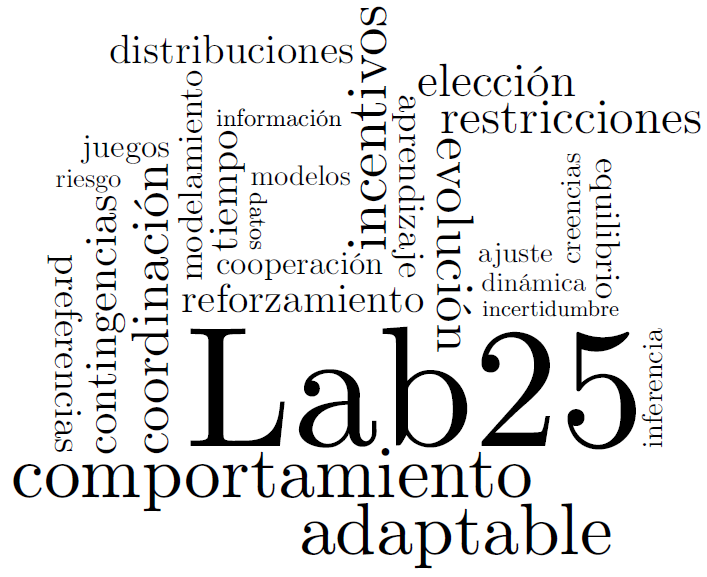
\includegraphics[width=12cm]{Figures/Lab25.png}};
\end{tikzpicture}



\begin{columns}[t] % The whole poster consists of three major columns, the second of which is split into two columns twice - the [t] option aligns each column's content to the top
\begin{column}{\sepwid}\end{column} % Empty spacer column
\begin{column}{\onecolwid} % The first column



%----------------------------------------------------------------------------------------
%   PRIMERA COLUMNA
%----------------------------------------------------------------------------------------
%   INTRODUCCION
%-------------------------------|||

\begin{alertblock}{Introduction: A memory phenomenon?}

Signal detection theory has been applied to Recognition Memory studies to describe subjects’ ability to discriminate between stimuli that have been presented before from a new set of stimuli (Wixted, 2007). When comparing subjects' performance between two classes of stimuli, one being more easily recognized (A) than the other (B), the response patterns obtained show that the difference in their discriminability  is reflected in the identification of both target and lure stimuli, suggesting that stimuli distributions involved move along the decision axis leading to its identification as the Mirror Effect, (Glanzer, Adams, Kim, 1993). 
\begin{figure}
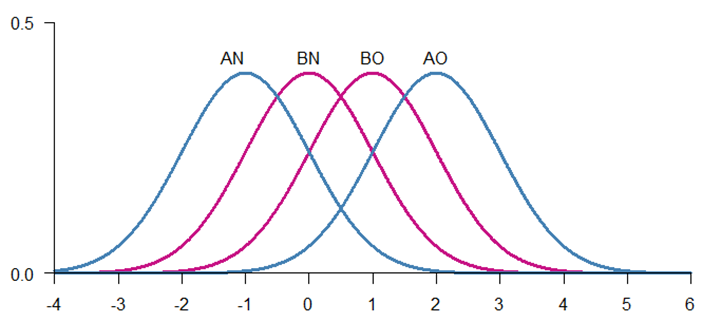
\includegraphics[width=0.5\linewidth]{Figures/MirrorEffect.png}
\end{figure}

Evidence in favor of the Mirror Effect has been reported across different SDT-alike procedures. In typical Yes/No tasks, the Mirror Effect appears as:

\begin{equation}
FalseAlarms(A) < FalseAlarms(B) < Hits(B) < Hits(A)
\label{eqn:Rates}
\end{equation}

When participants are asked to valuate how confident they felt while answering to each trial:

\begin{equation}
R(AN) < R(BN) < R(BS) < R(AS)
\label{eqn:Confidence}
\end{equation}

However, the Mirror Effect has only been studied within Recognition Memory and so, most theories and models proposed to explain it tend to do it in terms of high-level processes engaged in the study phase, (DeCarlo, 2007, Glanzer et. al, 1993). The main goal of the present study was to explore the existence of the Mirror Effect outside Recognition Memory, testing these assumptions. 
\end{alertblock}


%------------------------------------------------------------------------------------------
% METODO
%-----------------------------------------|||||

\setbeamercolor{block alerted title}{fg=white,bg=Periwinkle} % Titulo
\setbeamercolor{block alerted body}{fg=black,bg=white} % Cuerpo
\begin{alertblock}{Method: A perceptual task}

Two levels of perceptual discriminability constructed according to the literature on the Ebbinghaus illusion, (Massaro, 1971).

\begin{itemize}
\item High accuracy (A): Ebbinghaus illusions with 2 or 3 surrounding circles.
\item Low accuracy (B): Ebbinghaus illusions with 7 or 8 surrounding circles.
\end{itemize}


Detection task:  Are the two central circles of the same size?


Confidence Rate Task:  On a scale from 1 to 3, how confident are you of your response?


Two experiments: 

\begin{itemize}
\item Experiment 1: Just the right circle to compare is shown part of an Ebbinghaus illusion.
\item Experiment 2: Both circles were constructed as Ebbinghaus illusions.
\end{itemize}

Technical details: 

\begin{itemize}
\item 640 trials (total)
%	\item 340 - A condition |  340 - B condition
%		\item 160 - Noise | 160 - Signal
\item 40 different stimuli, (10 repetitions, at least)
%	\item 16 different noise stimuli per condition
%	\item 4 different signal stimuli per condition
%
\item Over and Underestimation trials
\item 1.5 s exposure
\item Space-bar between trials
\end{itemize}
\end{alertblock}

%-----------------------------------------------------------------------------------------
% FIN PRIMERA COLUMNA
%-----------------------------------------------------------------------------------------

\end{column} % End of the first column

\begin{column}{\sepwid}\end{column} % Empty spacer column

\begin{column}{\twocolwid} % Begin a column which is two columns wide (column 2)

\begin{columns}[t,totalwidth=\twocolwid] % Split up the two columns wide column

\begin{column}{\onecolwid}\vspace{-.6in} % The first column within column 2 (column 2.1)

%----------------------------------------------------------------------------------------
%   PROCEDIMIENTO
%-------------------------------||||||||

\setbeamercolor{block alerted title}{fg=white,bg=Periwinkle} % Titulo
\setbeamercolor{block alerted body}{fg=black,bg=white} % Cuerpo
\begin{alertblock}{Procedure: The actual task}

\begin{enumerate}
\item Detection Task:
\begin{center}
\begin{tabular}{ccc}
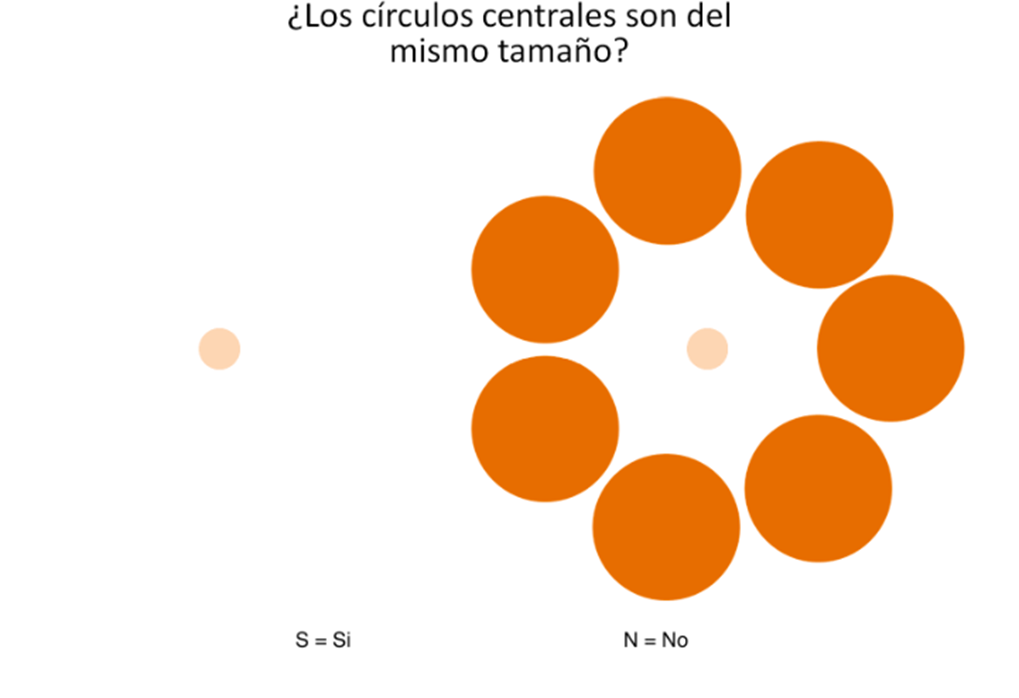
\includegraphics[width=0.45\linewidth]{Figures/MainTask.png} & \hfill & 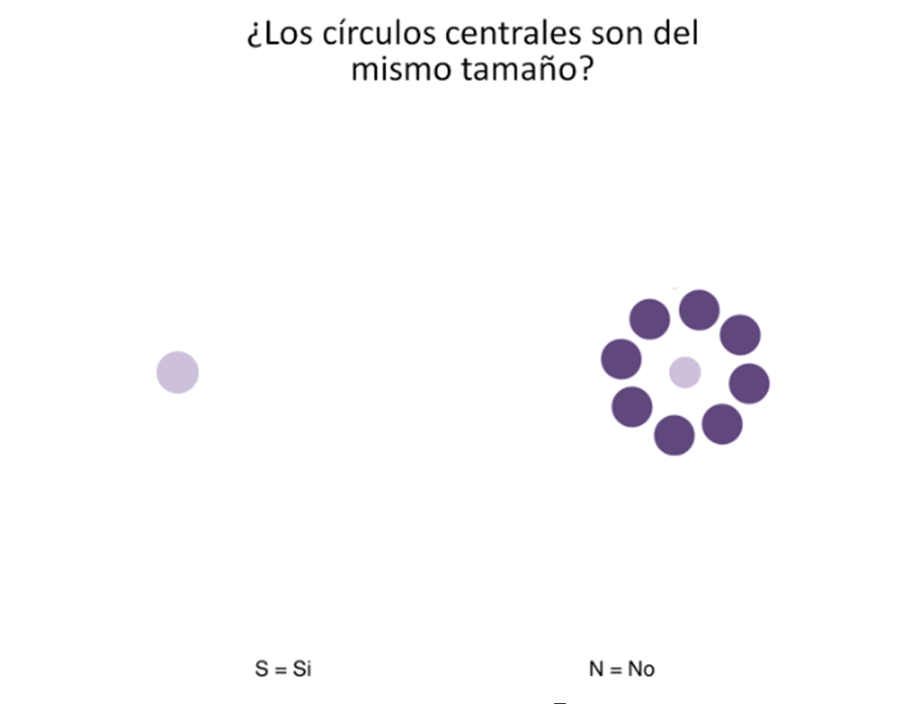
\includegraphics[width=0.4\linewidth]{Figures/MainTask2.png}
\end{tabular}
\end{center}
\item Confidence Rating
\begin{figure}
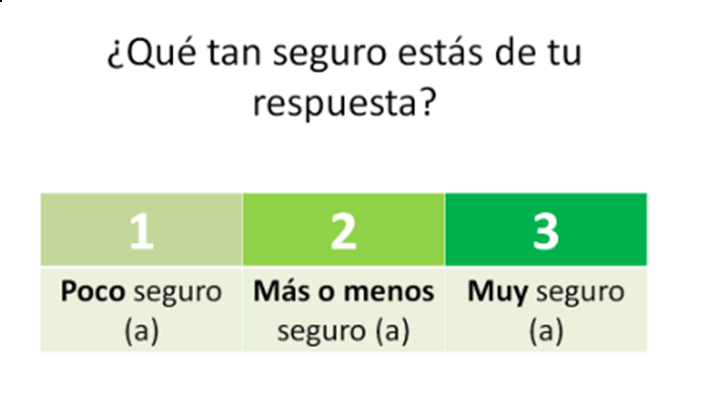
\includegraphics[width=0.5\linewidth]{Figures/ConfidenceTask.png}
\end{figure}
\end{enumerate}
\end{alertblock}
\end{column} % End of column 2.1
%----------------------------------------------------------------------------------------


\begin{column}{\twocolwid}\vspace{-.6in} % The second column within column 2 (column 2.2)

%----------------------------------------------------------------------------------------
%   METHODS
%----------------------------------------------------------------------------------------

\setbeamercolor{block alerted title}{fg=white,bg=RoyalBlue} % Change the alert block title colors
\setbeamercolor{block alerted body}{fg=black,bg=white} % Change the alert block body colors
\begin{alertblock}{Classical Analysis!}


\begin{center}
\begin{tabular}{ccc}
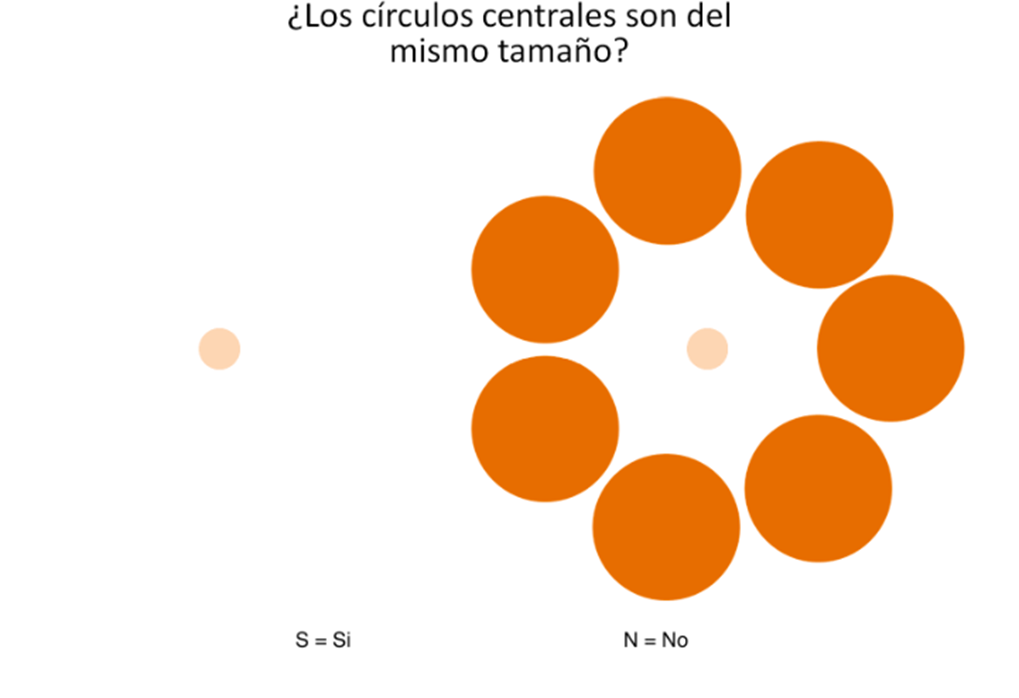
\includegraphics[width=0.55\linewidth]{Figures/MainTask.png} & \hfill & 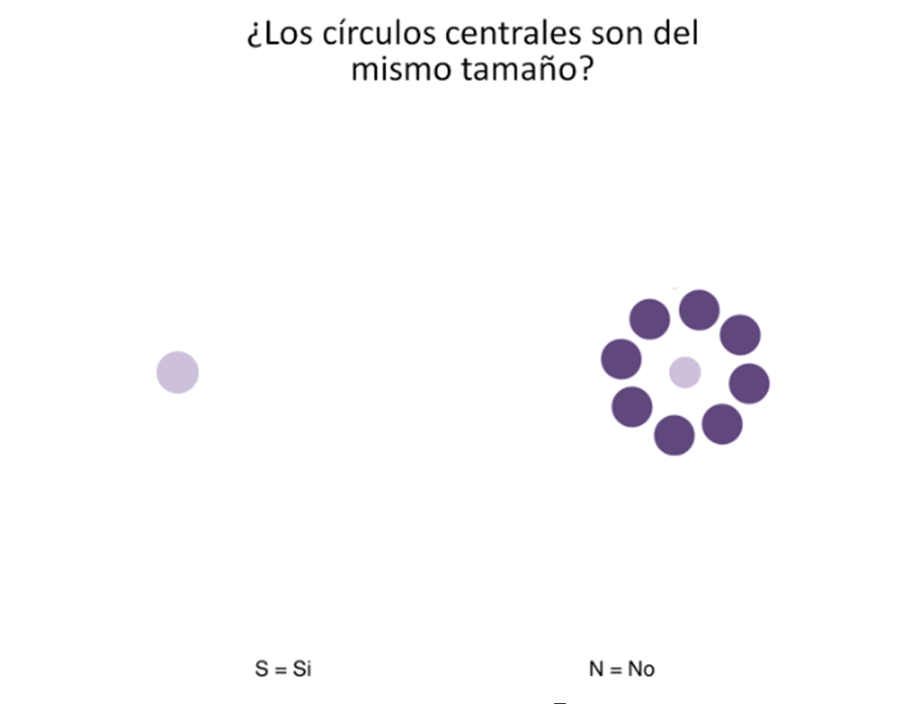
\includegraphics[width=0.5\linewidth]{Figures/MainTask2.png}
\end{tabular}
\end{center}


%Lorem ipsum dolor \textbf{sit amet}, consectetur adipiscing elit. Sed laoreet accumsan mattis. Integer sapien tellus, auctor ac blandit eget, sollicitudin vitae lorem. Praesent dictum tempor pulvinar. Suspendisse potenti. Sed tincidunt varius ipsum, et porta nulla suscipit et. Etiam congue bibendum felis, ac dictum augue cursus a. \textbf{Donec} magna eros, iaculis sit amet placerat quis, laoreet id est. In ut orci purus, interdum ornare nibh. Pellentesque pulvinar, nibh ac malesuada accumsan, urna nunc convallis tortor, ac vehicula nulla tellus eget nulla. Nullam lectus tortor, \textit{consequat tempor hendrerit} quis, vestibulum in diam. Maecenas sed diam augue.

\end{alertblock}

%----------------------------------------------------------------------------------------

\end{column} % End of column 2.2

\end{columns} % End of the split of column 2 - any content after this will now take up 2 columns width

%----------------------------------------------------------------------------------------
%   IMPORTANT RESULT
%----------------------------------------------------------------------------------------
\setbeamercolor{block alerted title}{fg=white,bg=RoyalBlue} % Change the alert block title colors
\setbeamercolor{block alerted body}{fg=black,bg=white} % Change the alert block body colors
\begin{alertblock}{What did we find? (Spoiler alert!)}

In both experiments, the pattern of responses identified as the Mirror Effect was found on at least 85\% of the participants.

\end{alertblock} 


\setbeamercolor{block alerted title}{fg=white,bg=Salmon} % Change the alert block title colors
\setbeamercolor{block alerted body}{fg=black,bg=white} % Change the alert block body colors
\begin{alertblock}{Bayesian Modeling}

In both experiments, the pattern of responses identified as the Mirror Effect was found on at least 85\% of the participants.

\end{alertblock} 



%----------------------------------------------------------------------------------------

\begin{columns}[t,totalwidth=\twocolwid] % Split up the two columns wide column again

\begin{column}{\onecolwid} % The first column within column 2 (column 2.1)

%----------------------------------------------------------------------------------------
%   MATHEMATICAL SECTION
%----------------------------------------------------------------------------------------

\begin{block}{Classical Data Analysis}

Nam quis odio enim, in molestie libero. Vivamus cursus mi at nulla elementum sollicitudin. Nam quis odio enim, in molestie libero. Vivamus cursus mi at nulla elementum sollicitudin.

\begin{equation}
\kappa =\frac{\xi}{E_{\mathrm{max}}} %\mathbb{ZNR}
\end{equation}

\end{block}

%----------------------------------------------------------------------------------------

\end{column} % End of column 2.1

\begin{column}{\onecolwid} % The second column within column 2 (column 2.2)

%----------------------------------------------------------------------------------------
%   RESULTS
%----------------------------------------------------------------------------------------

\begin{block}{Results}

\begin{table}
\vspace{2ex}
\begin{tabular}{l l l}
\toprule
\textbf{Treatments} & \textbf{Response 1} & \textbf{Response 2}\\
\midrule
Treatment 1 & 0.0003262 & 0.562 \\
Treatment 2 & 0.0015681 & 0.910 \\
Treatment 3 & 0.0009271 & 0.296 \\
\bottomrule
\end{tabular}
\caption{Table caption}
\end{table}

\end{block}

%----------------------------------------------------------------------------------------

\end{column} % End of column 2.2

\end{columns} % End of the split of column 2

\end{column} % End of the second column

\begin{column}{\sepwid}\end{column} % Empty spacer column

\begin{column}{\onecolwid} % The third column

%----------------------------------------------------------------------------------------
%   CONCLUSION
%----------------------------------------------------------------------------------------

\begin{block}{Conclusion}

The present study is the first to show evidence for the existence of the Mirror Effect patterns of response, on a signal detection task that does not involve recognition memory. The perceptual task here presented lacked of a pre-experimental phase where participants had the chance to manipulate how powerful the illusions included in each condition were, contradicting what has been proposed within recognition memory studies. The fact that the Mirror Effect was found on a perceptual task, with accuracy conditions designed specifically in terms of the signal that participants are asked to detect, may suggest that there’s a much more basic principle regulating the patterns of response observed.

\end{block}

%----------------------------------------------------------------------------------------
%   ADDITIONAL INFORMATION
%----------------------------------------------------------------------------------------

\begin{block}{Additional Information}

Maecenas ultricies feugiat velit non mattis. Fusce tempus arcu id ligula varius dictum. 
\begin{itemize}
\item Curabitur pellentesque dignissim
\item Eu facilisis est tempus quis
\item Duis porta consequat lorem
\end{itemize}

\end{block}

%----------------------------------------------------------------------------------------
%   REFERENCES
%----------------------------------------------------------------------------------------

\begin{block}{References}

\nocite{*} % Insert publications even if they are not cited in the poster
\small{\bibliographystyle{unsrt}
\bibliography{sample}\vspace{0.75in}}

\end{block}

%----------------------------------------------------------------------------------------
%   ACKNOWLEDGEMENTS
%----------------------------------------------------------------------------------------

\setbeamercolor{block title}{fg=red,bg=white} % Change the block title color

\begin{block}{Acknowledgements}

\small{\rmfamily{First of all, }} \\

\end{block}

%----------------------------------------------------------------------------------------
%   CONTACT INFORMATION
%----------------------------------------------------------------------------------------

\setbeamercolor{block alerted title}{fg=black,bg=norange} % Change the alert block title colors
\setbeamercolor{block alerted body}{fg=black,bg=white} % Change the alert block body colors

\begin{alertblock}{Contact Information}

\begin{itemize}
\item Web: \href{http://www.university.edu/smithlab}{http://www.university.edu/smithlab}
\item Email: \href{mailto:john@smith.com}{john@smith.com}
\item Phone: +1 (000) 111 1111
\end{itemize}

\end{alertblock}


%----------------------------------------------------------------------------------------

\end{column} % End of the third column
\end{columns} % End of all the columns in the poster
\end{frame} % End of the enclosing frame
\end{document}

              